\documentclass{article}
\usepackage{v-test-paper}

%\renewcommand{\ans}{\quad}
%\def\ansint#1{\quad}

\title{Module-Test-10\\(Physics-JEE)}
\begin{document}

\maketitle

\jeeSectionA
\begin{enumerate}
\item A $2 \kg$ block slides on a horizontal floor with a speed of $4 \mps$. It strikes a uncompressed spring and compresses it till the block is motionless. The kinetic friction force is $15 \N$ and spring constant is $10000 \N/\m$. The spring compresses by
\begin{center}
\begin{tikzpicture}
	\fill[pattern=north east lines](0, 0)--(7.75, 0)--(7.75, 1.5)--(8, 1.5)--(8, -0.25)--(0, -0.25)--cycle;
	\draw[thick](0, 0)--(7.75, 0)--(7.75, 1.5);
	\node[block] (block) at (2, 0.4) {$m$};
	\tzline+[->](block.east)(1, 0){$v$}[r]
	\tzsnake{5pt}[coil, amplitude=5pt, pre length=0pt](4.5,0.4){$k$}[a=2mm](7.75,0.4)
\end{tikzpicture}
\end{center}
\begin{tasks}(2)
	\task $5.5\cm$ \ans
	\task $2.5\cm$ 
	\task $11.0\cm$
	\task $8.5\cm$
\end{tasks}

\item An open knife of mass $m$ is dropped from a height $h$ on a wooden floor. If the blade penetrates up to the depth $d$ into the wood, the average resistance offered by the wood to the knife edge is
\begin{tasks}(2)
	\task $mg\left( 1+\dfrac{h}{d} \right)$\ans
	\task $mg\left( 1+\dfrac{h}{d} \right)^2$
	\task $mg\left( 1-\dfrac{h}{d} \right)$
	\task $mg\left( 1+\dfrac{d}{h} \right)$
\end{tasks}

\item A vertical spring is fixed to one of its end and a massless plank fitted to the other end.
A block is released from a height $h$ as shown. Spring is in relaxed position. Then choose the correct statement.
\begin{center}
\begin{tikzpicture}
	\pic (surface) {frame=3cm};
	\node[fplatform] (platform) at (0, 2.5) {};
	\node at (platform.center)[fill=white, inner sep=1pt, scale=0.75]{massless};
	\tzsnake{5pt}[coil, amplitude=5pt](surface-center){$k$}[r=2mm](platform.south)
	\node[block, yshift=1cm] (block) [above of=platform] {$m$};
	\tzline[|<->|]<1, 0>(platform.north)(block.south){$h$}[r, midway]
\end{tikzpicture}
\end{center}
\begin{tasks}(1)
	\task The maximum compression of the spring does not depend on $h$
	\task The maximum kinetic energy of the block does not depend on $h$
	\task The compression of the spring at maximum $K.E.$ of the block does not depend on $h$\ans
	\task The maximum compression of the spring does not depend on $k$
\end{tasks}

\item A spring of force constant $800 \N/\m$ has an extension of $5 \cm$. The work done in extending it from $5 \cm$ to $15 \cm$ is
\begin{tasks}(2)
	\task $16\Joule$
	\task $8\Joule$\ans
	\task $32\Joule$
	\task $24\Joule$
\end{tasks}

\item A block of mass $m$ is kept on a platform which starts from rest with constant acceleration $\dfrac{g}{2}$ upwards as shown in figure. Work done by normal reaction on block in time $t$ is
\begin{center}
\begin{tikzpicture}
	\pic {frame=5cm};
	\node[fplatform] at (0, 0.2){};
	\node[block] at (0, 0.8) {$m$};
	\tzline[->] (2, 0.5)(2, 2){$\dfrac{g}{2}$}[r, midway]
\end{tikzpicture}
\end{center}
\begin{tasks}(2)
	\task $\dfrac{mg^2t^2}{8}$
	\task $\dfrac{3mg^2t^2}{8}$\ans
	\task $0$
	\task $-\dfrac{mg^2t^2}{8}$
\end{tasks}

\item A force $F=-k(yi+xj)$ (where, $k$ is a positive constant) acts on a particle moving in the x-y plane. Starting from the origin, the particle is taken along the positive X-axis to the point $(a,0)$ and then parallel to the Y-axis to the point $(a, a)$. The total work done by the force $F$ on the particle is
\begin{tasks}(2)
	\task $-2ka^2$
	\task $2ka^2$
	\task $-ka^2$\ans
	\task $ka^2$
\end{tasks}

\item The relationship between the force $F$ and position $x$ of a body is as shown in figure. The work done in displacing the body from $x = 1\m$ to $x = 5\m$ will be
\begin{center}
\begin{tikzpicture}[yscale=0.3]
	\tzaxes(-0.5, -7)(8, 12){$x$}{$F$}
	\tzlines(0, 0)(1, 10)(2, 10)(2, 5)(3, 5)(3, -5)(4, -5)(4, 0)(5, 10)(5, 0)(6, 0)(6, 5)(7, 5);
	\tzticks(-1pt:1pt){1/$1$,2/$2$,3/$3$, 4/$4$, 5/$5$, 6/$6$, 7/$7$}(-1pt:1pt)
        {-5/$-5$,5/$5$,10/$10$}
    \tzproj[dashed, red](1,10)
    \tzproj[dashed, red](2,5)
    \tzprojx[dashed,red](7,5)
    \tzprojy[dashed, red](3,-5)
\end{tikzpicture}
\end{center}
\begin{tasks}(2)
	\task $30\Joule$
	\task $15\Joule$\ans
	\task $25\Joule$
	\task $20\Joule$
\end{tasks}

\item If $W_1$, $W_2$ and $W_3$ represent the work done in moving a
particle from $A$ to $B$ along three different paths $1$, $2$ and $3$ respectively (as shown) in the gravitational field of a point mass $m$. Find the correct relation between $W_1$ , $W_2$ and $W_3$.
\begin{center}
\begin{tikzpicture}
	\tzdot*(0, 0){$A$}[l]
	\tzdot*(2, 2){$B$}[r]
	\tzline[-->--](0, 0)(0, 2){$W_1$}[l]
	\tzline[-->--](0, 2)(2, 2)
	\tzline[-->--](0, 0){$W_2$}[l=2mm](2, 2)
	\tzto[bend right,-->--](0,0)(2,2)
	\tznode(1.5, 0.8){$W_3$}[r]
\end{tikzpicture}
\end{center}
\begin{tasks}(2)
	\task $W_1 > W_2 > W_3$
	\task $W_1 = W_2 = W_3$\ans
	\task $W_1 < W_2 < W_3$
	\task $W_2 > W_1 > W_3$
\end{tasks}

\item A force acts on a $2 \kg$ object, so that its position is given as a function of time as $x = 3t^2 + 5$. What is the work done by this force in first 5 seconds?
\begin{tasks}(2)
	\task $850\Joule$ 
	\task $900\Joule$ \ans 
	\task $950\Joule$
	\task $875\Joule$
\end{tasks}

\item A particle moves in one dimension from rest under the influence of a force that varies with the distance travelled by the particle as shown in the figure. The kinetic energy of the particle after it has travelled $3 \m$ is
\begin{center}
\begin{tikzpicture}
	\tzaxes(-0.5, -0.5)(5, 4){$x$}{$F$}
	\tzlines(0, 2)(2, 2)(3, 3);
	\tzticks(-1pt:1pt){1/$1$,2/$2$,3/$3$}(-1pt:1pt)
        {1/$1$,2/$2$,3/$3$}
    \tzproj[dashed, red](3,3)
    \tzprojx[dashed,draw=red](2,2)
\end{tikzpicture}
\end{center}
\begin{tasks}(2)
	\task $4\Joule$
	\task $2.5\Joule$
	\task $6.5\Joule$\ans
	\task $5\Joule$
\end{tasks}

\item A time dependent force $F = 6t$ acts on a particle of mass
$1 \kg$. If the particle starts from rest, the work done by the force during the first $1 \s$ will be
\begin{tasks}(2)
	\task $22\Joule$
	\task $9\Joule$
	\task $18\Joule$
	\task $4.5\Joule$\ans
\end{tasks}

\item A particle which is experiencing a force, is given by $\vec{F}=3\hat{i}-12\hat{j}$, undergoes a displacement of $\vec{d}=4\hat{i}$. If the particle had a kinetic energy of $3\Joule$ at the beginning of the displacement, what is its kinetic energy at the end of the displacement ?
\begin{tasks}(2)
	\task $9\Joule$
	\task $15\Joule$\ans
	\task $12\Joule$
	\task $10\Joule$
\end{tasks}

\item Two masses of $1\gm$ and $4\gm$ are moving with equal kinetic energies. The ratio of the magnitudes of their momenta is
\begin{tasks}(2)
	\task $4:1$
	\task $\sqrt{2}:1$
	\task $1:2$\ans
	\task $1:16$
\end{tasks}

\item A body of mass $m=10^{-2}\kg$ is moving in a medium and experiences a frictional force $F=-kv^2$. Its initial speed is $v_0=10\mps$. If, after $10\s$, its energy is $\dfrac{1}{8}mv_0^2$, the value of $k$ will be
\begin{tasks}(2)
	\task $10^{-3}\kg/\s$
	\task $10^{-4}\kg/\m$\ans
	\task $10^{-1}\kg/\m\s$
	\task $10^{-3}\kg/\m$
\end{tasks}

\item A projectile is fired from the origin with a velocity $v_0$ at an angle $\theta$ with the x-axis. The speed of the projectile at an altitude $h$ is
\begin{tasks}(2)
	\task $v_0\cos\theta$
	\task $\sqrt{v_0^2-2gh}$\ans
	\task $\sqrt{v_0^2\sin^2\theta-2gh}$
	\task None of these
\end{tasks}

\item A particle moves under the action of a force $F = 20\hat{i} + 15 \hat{j}$ along a straight line $3y + \alpha x = 5$, where, $\alpha$ is a constant. If the work done by the force $F$ is zero, then the value of $\alpha$ is
\begin{tasks}(2)
	\task $\dfrac{4}{9}$
	\task $\dfrac{9}{4}$
	\task $3$
	\task $4$\ans
\end{tasks}


\item A mass of $0.5 \kg$ moving with a speed of $1.5 \mps$ on a horizontal smooth surface, collides with a nearly weightless spring of force constant $k = 50 \N/\m$. The maximum compression of the spring would be
\begin{tasks}(2)
	\task $0.15\m$\ans
	\task $0.12\m$
	\task $0.5\m$
	\task $0.25\m$
\end{tasks}



\item At time $t = 0$ , particle starts moving along the
x-axis. If its kinetic energy increases uniformly with time $t$ , the net force acting on it must be proportional to
\begin{tasks}(2)
	\task $\sqrt{t}$
	\task constant
	\task $t$
	\task $\dfrac{1}{\sqrt{t}}$\ans
\end{tasks}

\item A block of mass $m$ is connected to a spring of force constant $k$. Initially the block is at rest and the spring has natural length. A constant force $F$ is applied horizontally towards right. The maximum speed of the block will be (there is no friction between block and the surface)
\begin{center}
\begin{tikzpicture}
	\fill[pattern=north east lines](-0.25, -0.25)--(-0.25, 1.5)--(0, 1.5)--(0, 0)--(6, 0)--(6, -0.25)--cycle;
	\draw[thick](0, 1.5)--(0, 0)--(6, 0);
	\node[block] (block) at (3, 0.4) {$m$};
	\tzline+[->](block.east)(1, 0){$F$}[r]
	\tzsnake{5pt}[coil, amplitude=5pt](0,0.4){$k$}[a=2mm](block.west)
\end{tikzpicture}
\end{center}
\begin{tasks}(2)
	\task $\dfrac{F}{\sqrt{2mk}}$
	\task $\dfrac{F}{\sqrt{mk}}$\ans
	\task $\dfrac{\sqrt{2}F}{\sqrt{mk}}$
	\task $\dfrac{2F}{\sqrt{mk}}$
\end{tasks}

\item A block tied between two identical springs is in equilibrium. If upper spring is cut, then
the acceleration of the block just after cut is $5 \mpss$. Now if instead of upper string lower spring is cut, then the acceleration of the block just after the cut will be
(Take $g = 10 \mpss$)
\begin{center}
\begin{tikzpicture}
	\pic[rotate=-180] (ceiling) {frame=2cm};
	\pic[rotate=0] (surface)at (0, -5) {frame=2cm};
	\node[block] (block) at (0, -2.5) {$m$};
	\tzsnake{5pt}[coil, amplitude=5pt](ceiling-center)(block.north)
	\tzsnake{5pt}[coil, amplitude=5pt](surface-center)(block.south)
\end{tikzpicture}
\end{center}
\begin{tasks}(2)
	\task $1.25\mpss$
	\task $5\mpss$\ans
	\task $10\mpss$
	\task $2.5\mpss$
\end{tasks}




\end{enumerate}

\jeeSectionB
\begin{enumerate}\addtocounter{enumi}{20}

\item A ball of mass $1 \kg$ is dropped from a tower. Find power of gravitational force at time $t = 2 \s$. Take $g = 10 \mpss$.\ansint{200}

\item A block of mass $5 \kg$ is raised from the bottom of the lake to a height of $3 \m$ without change in kinetic energy. If the density of the block is $3000 \kg/\m^3$ , then the work done is equal to \ansint{100}

\item A body is displaced from origin to $(1\m,1\m)$ by a force $\vec{F}=2y\hat{i} + 3x^2\hat{j}$ along the path $y=x^2$, if the work done along the path is $W$ then $[W]$ is (where $[\; ]$ is greatest integer function) \ansint{2}

\item Two masses $m_1 = 10 \kg$ and $m_2 = 5 \kg$ are connected by an ideal string as shown in the figure. The coefficient of friction between $m_1$ and the surface is $\mu = 0.2$. Assuming that the system is released from rest. Calculate the velocity of blocks when $m_2$ has descended by $4 \m$. ($g = 10 \mpss$) \ansint{4}
\begin{center}
\begin{tikzpicture}
\def\ph{0.6}
	\fill[pattern=north east lines](0, 0)--(8, 0)--(8, -3)--(7.75, -3)--(7.75, -0.25)--(0, -0.25)--cycle;
	\draw[thick](0, 0)--(8, 0)--(8, -3);
	\node[spulley] (pulley) at (8+\ph*cos{45}, \ph){};
	
	\node[vblock] (block1) at (3, 1){$m_1$};
	\tzline(pulley.center)(8, 0)
	\tzdot*(pulley.center)
	\node[block, ] (block2) at ($(pulley.east) + (0, -2)$){$m_2$};
	\tzline(pulley.east)(block2.north)
	\tzline(pulley.north)(block1.east)
	\tzlines[->](0, 0.5){$\mu$}[a](1, 0.5)(1.5, 0);
\end{tikzpicture}
\end{center}

\item In the figure shown, all surfaces are smooth and force constant of spring is $10 \N/\m$. Block of mass $2 \kg$ is not attached with the spring. The spring is compressed by $2\m$ and then released. Find the maximum distance $d$ travelled by the block over the inclined plane. Take ($g = 10 \mpss$) .\ansint{2}
\begin{center}
\begin{tikzpicture}
	\fill[pattern=north east lines](-0.25, -0.25)--(-0.25, 1.5)--(0, 1.5)--(0, 0)--(6, 0)--(8.6, 1.5)--(8.6, -0.25)--cycle;
	\draw[thick](0, 1.5)--(0, 0)--(6, 0)--(8.6, 1.5);
	\node[block] (block) at (3, 0.4) {$m$};
	\tzline+[->](block.east)(1, 0){$v$}[r]
	\tzsnake{5pt}[coil, amplitude=5pt, pre length=5pt, post length=0pt](0,0.4){$k$}[a=2mm](block.west)
	\tzanglemark[thick, ->](8.6, 0)(6, 0)(8.6, 1.5){$30^\circ$}[fill=white, inner sep=1pt](25pt)
	\tzline+[dashed](6, 0)(2, 0)
\end{tikzpicture}
\end{center}



\item A rod of length $1.0 \m$ and mass $1 \kg$ fixed at one end is initially hanging vertical. The other end is now raised until it makes an angle $90^\circ$ with the vertical. How much work is required ? ($g=10\mpss$) \ansint{5}

\item In the given figure, system is released from rest. Friction is absent and string is massless. In time $t=0.3\s$, work done by gravity on $2\kg$ block is ($g=10\mpss$) \ansint{3}
\begin{center}
\begin{tikzpicture}
	\pic[rotate=-180] (ceiling) {frame=3cm};
	\node[pulley] (pulley) at ($(ceiling-center)+(0, -1)$) {};
	\tzdot*(pulley.center)
	\tzline(pulley.center)(ceiling-center)
	\node[block] (block1) at ($(pulley.west)+(0, -2)$) {$1\kg$};
	\node[block] (block2) at ($(pulley.east)+(0, -2.5)$) {$2\kg$};
	\tzline(pulley.east)(block2.north)
	\tzline(pulley.west)(block1.north)
\end{tikzpicture}
\end{center}

\item For the given graph find the work done by the force.\ansint{4}
\begin{center}
\begin{tikzpicture}
	\tzaxes(-0.5, -0.5)(5, 3){$x$}{$F$}
	\tzticks(-1pt:1pt){1/$1$, 2/$2$, 3/$3$, 4/$4$}(-1pt:1pt){1/$1$, 2/$2$}
	\tzlines(0, 0)(2, 2)(4, 0);
	\tzproj[dashed, red](2,2)
\end{tikzpicture}
\end{center}

\item Suppose you drag a block slowly of mass $1\kg$ on a horizontal rough plane for $2\m$ by applying a force of $5\N$, then find the magnitude of work done by the friction force. \ansint{10}

\item A force $F = (2 + 2x)$ acts on a particle in x-direction where $F$ is in newton and $x$ in metre. Find the work done by this force during a displacement from $x = 1.0 \m$ to $x = 2.0 \m$.\ansint{5}


\end{enumerate}

\end{document}